\documentclass[tikz,border=10pt]{standalone}
\usepackage{amsmath}
\usetikzlibrary{angles,quotes}
\begin{document}
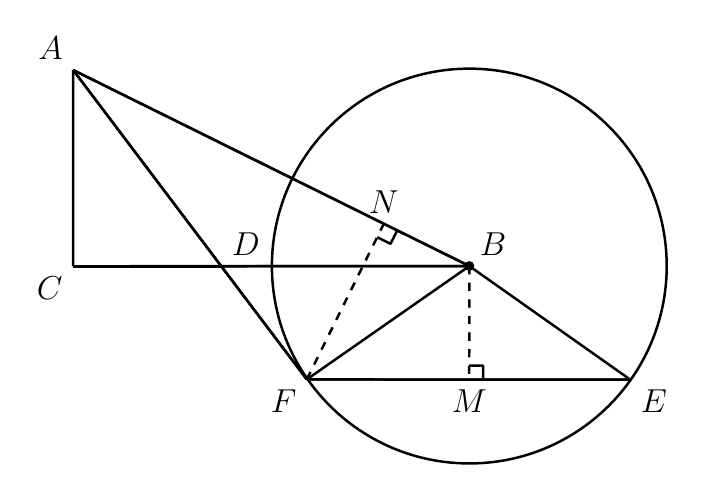
\begin{tikzpicture}[line width=0.9pt, line join=round, font=\fontsize{11.5}{13.8}\selectfont]
\coordinate (A) at (-3.559,2.364);
\coordinate (B) at (1.472,-0.125);
\coordinate (C) at (-3.561,-0.128);
\coordinate (D) at (-1.678,-0.128);
\coordinate (E) at (3.518,-1.569);
\coordinate (F) at (-0.592,-1.565);
\coordinate (M) at (1.471,-1.567);
\coordinate (N) at (0.386,0.412);




\draw (A) -- (B);
\draw (A) -- (C);
\draw (A) -- (D);
\draw (A) -- (F);
\draw (A) -- (N);
\draw (N) -- (B);
\draw (B) -- (C);
\draw (C) -- (D);
\draw (D) -- (B);
\draw (D) -- (F);
\draw (B) -- (E);
\draw (B) -- (F);
\draw (F) -- (M);
\draw (M) -- (E);
\draw (E) -- (F);


\draw (B) circle[radius=2.507];


\draw[dashed] (F) -- (N);
\draw[dashed] (B) -- (M);


\draw pic[draw, angle radius=0.176cm] {right angle=B--M--E};
\draw pic[draw, angle radius=0.190cm] {right angle=B--N--F};


\fill (B) circle[radius=1.800pt];


\node[above left] at (A) {$A$};
\node[below left] at (C) {$C$};
\node[above right] at (D) {$D$};
\node[above right] at (B) {$B$};
\node[above] at (N) {$N$};
\node[below left] at (F) {$F$};
\node[below] at (M) {$M$};
\node[below right] at (E) {$E$};
\end{tikzpicture}
\end{document}